% monty_hall_fsm.tex
\documentclass[11pt]{article}

\usepackage[margin=1in]{geometry}
\usepackage{microtype}
\usepackage{graphicx}
\usepackage{booktabs}
\usepackage{caption}
\usepackage{hyperref}

\title{Monty Hall as a Finite State Machine}
\author{Jeremy Evert}
\date{\today}

\begin{document}
\maketitle

\section{Overview}
This document models the Monty Hall game as a finite state machine (FSM).
We generate the diagram programmatically using Graphviz (DOT) and include the resulting PDF directly in \LaTeX.

\section{FSM Diagram}
Figure~\ref{fig:monty-hall-fsm} is auto-generated from \texttt{monty\_hall\_fsm.dot}.

\begin{figure}[h!]
  \centering
  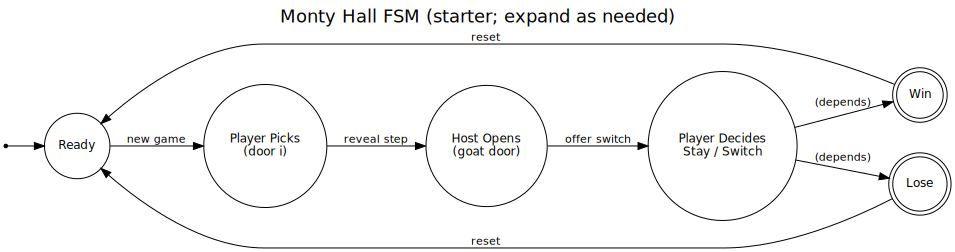
\includegraphics[width=\linewidth]{monty_hall_fsm.pdf}
  \caption{Monty Hall FSM (Graphviz-generated).}
  \label{fig:monty-hall-fsm}
\end{figure}

\section{Notes (for later refinement)}
You can evolve this FSM toward \textit{about 15 states} by:
\begin{itemize}
  \item encoding hidden state (car placement) explicitly,
  \item encoding player choice states,
  \item modeling host action as either a separate step or as labeled transitions,
  \item optionally adding probabilities to edges for the random parts.
\end{itemize}

\end{document}

